\documentclass[aspectratio=169]{beamer}

\usepackage[T1]{fontenc}
\usepackage[utf8]{inputenc}
\usepackage{amsmath, amssymb, amsfonts}
\usepackage{booktabs}
\usepackage{graphicx}

\usetheme{default}
\usecolortheme{default}
\setbeamertemplate{navigation symbols}{}
\setbeamertemplate{footline}{%
  \leavevmode%
  \makebox[\paperwidth][s]{%
    \hspace*{0.5cm}\insertshorttitle\hfill\insertframenumber{} / \inserttotalframenumber\hspace*{0.5cm}}%
  \vspace{4pt}%
}

\graphicspath{{../paper/figures/}}

\title[A Differentiable Atari VCS]{A Differentiable Atari VCS}
\subtitle{A Complex, Fully Known Ground Truth for Explainable AI}
\author{Anonymous Submission}
\date{AAAI-27 --- Supplementary Video}

\begin{document}

% ---- Page 1 : Title (segment 1) ----
\begin{frame}[plain]
  \titlepage
  \vfill
  \begin{center}
  \footnotesize A real computer architecture, made fully differentiable\\
  Two ports, bit-exact on all 64 Atari games\\
  Gradients with a ground truth
  \end{center}
\end{frame}

% ---- Page 2 : Motivation (segment 2) ----
\begin{frame}{Explanation needs ground truth}
  \begin{itemize}\setlength\itemsep{0.5em}
    \item To check an explanation, we must know the true mechanism
    \item Simple models: mechanism known, but explaining it tests nothing
    \item Deep networks: explanation needed, but no inner ground truth
    \item So an explanation can be confident and wrong
    \item We want a system that is complex, fully known, and differentiable
  \end{itemize}
\end{frame}

% ---- Page 3 : The Atari VCS idea (segment 3) ----
\begin{frame}{A study object: the Atari 2600}
  \begin{columns}
    \begin{column}{0.52\textwidth}
      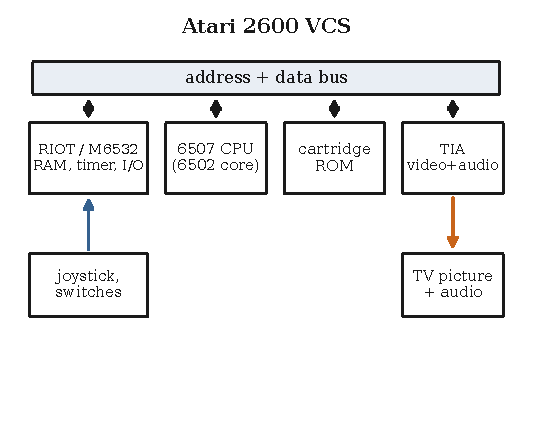
\includegraphics[width=\linewidth]{fig_architecture.pdf}
    \end{column}
    \begin{column}{0.46\textwidth}
      \begin{itemize}\setlength\itemsep{0.5em}
        \item A real 1977 computer: CPU, RAM, graphics chip, cartridge
        \item The platform that launched deep reinforcement learning
        \item Complex, yet fully specified to the last bit
        \item We re-express its every step so gradients can flow
      \end{itemize}
    \end{column}
  \end{columns}
\end{frame}

% ---- Page 4 : Two bit-exact ports (segment 4) ----
\begin{frame}{Two independent differentiable ports}
  \centering
  \setlength{\tabcolsep}{8pt}
  \begin{tabular}{lcc}
    \toprule
     & \textsc{jutari} & \textsc{jaxtari} \\
    \midrule
    Language / AD          & Julia / Zygote & JAX / XLA \\
    RAM-exact (of 64)      & \textbf{64}    & \textbf{64} \\
    Pixel-exact (of 64)    & \textbf{64}    & \textbf{64} \\
    Single env, CPU        & fastest        & vmap-batched \\
    Batched on GPU         & ---            & $\sim$3M steps/s \\
    \bottomrule
  \end{tabular}

  \vspace{1.2em}
  \begin{itemize}\setlength\itemsep{0.4em}
    \item Built twice, in two languages, against one reference
    \item Both match \textsc{xitari} bit-for-bit on all 64 games
  \end{itemize}
\end{frame}

% ---- Page 5 : Soft equals Hard (segment 7) ----
\begin{frame}{Soft equals hard}
  \centering
  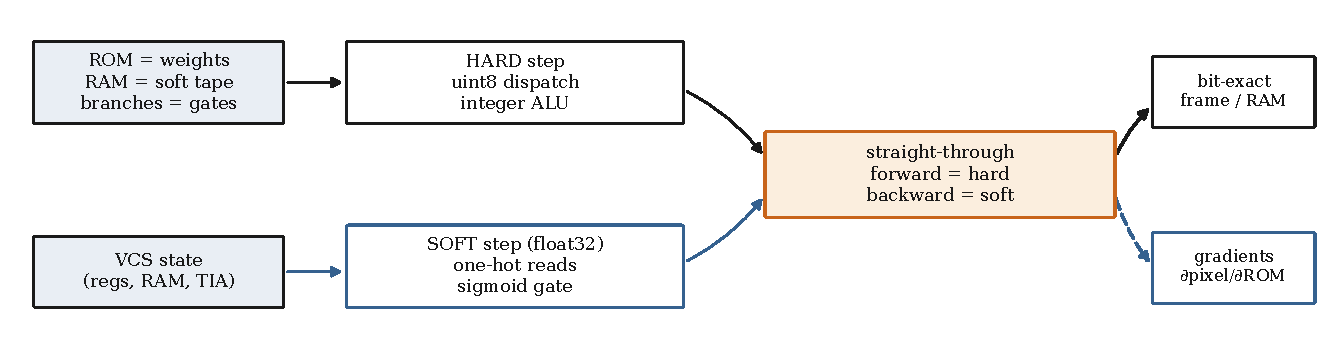
\includegraphics[width=0.82\linewidth]{fig_pipeline.pdf}
  \vspace{0.6em}
  \begin{itemize}\setlength\itemsep{0.35em}
    \item ROM as a weight tensor, RAM as a soft tape, branches as gates
    \item Forward pass is bit-exact equal to the hard machine
    \item Backward pass gives surrogate gradients where bits have none
  \end{itemize}
\end{frame}

% ---- Page 6 : GPU throughput (segment 9) ----
\begin{frame}{Throughput: a GPU path}
  \begin{columns}
    \begin{column}{0.6\textwidth}
      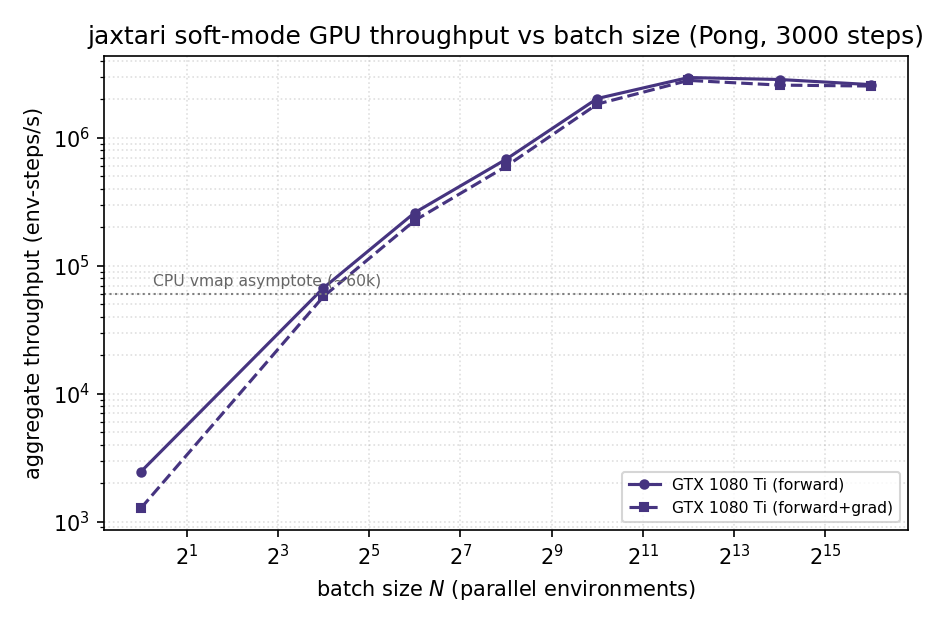
\includegraphics[width=\linewidth]{gpu_throughput.png}
    \end{column}
    \begin{column}{0.38\textwidth}
      \begin{itemize}\setlength\itemsep{0.5em}
        \item \textsc{jutari}: fastest per environment on CPU
        \item \textsc{jaxtari}: batches the rollout on a GPU
        \item Millions of environment-steps per second
        \item Gradients cost only a few percent more
      \end{itemize}
    \end{column}
  \end{columns}
\end{frame}

% ---- Page 7 : XAI proof of concept (segment 10) ----
\begin{frame}{Gradients with a ground truth}
  \centering
  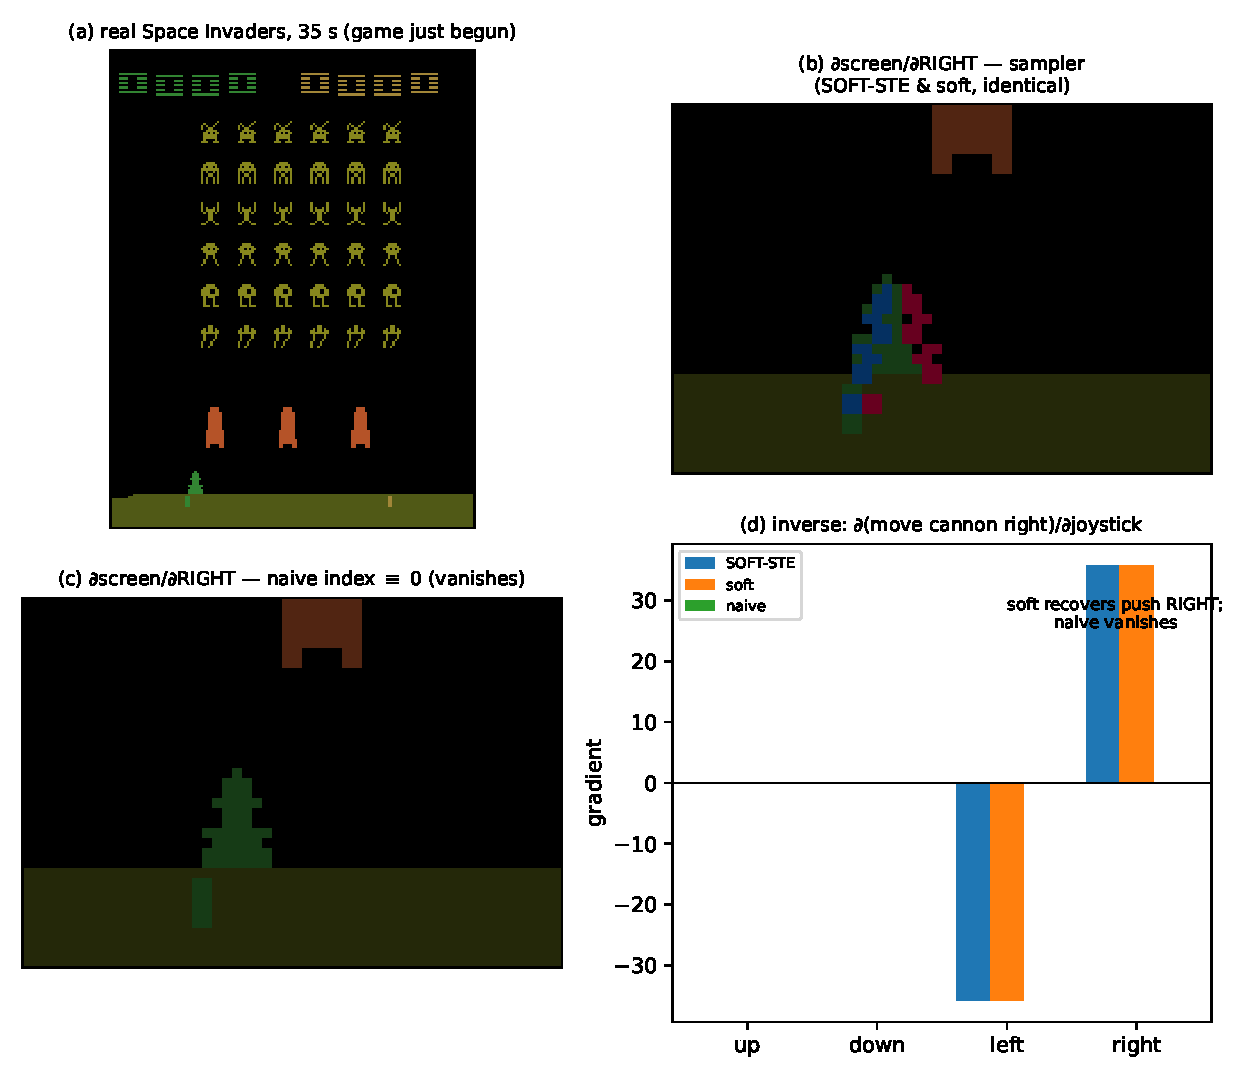
\includegraphics[width=0.95\linewidth]{si_joystick_gradient.pdf}
  \vspace{0.4em}
  \begin{itemize}\setlength\itemsep{0.3em}
    \item A real Space Invaders ROM, run in the differentiable substrate
    \item Gradient of the screen with respect to the joystick action
    \item An attribution that can be scored against the true mechanism
  \end{itemize}
\end{frame}

% ---- Page 8 : In the supplement (segment 11) ----
\begin{frame}{In the supplementary material}
  \begin{itemize}\setlength\itemsep{0.5em}
    \item Full proofs of the forward-equivalence and temperature-limit results
    \item A study of how the relaxation parameters shape the gradient
    \item Every game, with its ROM hash, mapper, and per-frame exactness
    \item Throughput tables for CPU and GPU
    \item These side-by-side comparison videos
  \end{itemize}
\end{frame}

% ---- Page 9 : Conclusion (segment 12) ----
\begin{frame}{A testbed for explainable AI}
  \begin{itemize}\setlength\itemsep{0.5em}
    \item A complex system that is fully known and fully differentiable
    \item Built twice, validated bit-for-bit on all 64 games
    \item Exact frames, with surrogate gradients for attribution
    \item The XAI ground truth we hope the community takes up
  \end{itemize}
  \vfill
  \begin{center}
  \small Full code of both ports released under the MIT license upon acceptance.\\
  Thank you.
  \end{center}
\end{frame}

\end{document}
